\section{Аппроксимация байесовского классификатора}\label{sec:ch1/bayesian_classifier_approximation}

Для построения классификатора, приближающего оптимальное байесовское правило, предполагается наличие размеченного обучающего набора \((X, Y) = \{(X_1, Y_1), \dots, (X_n, Y_n)\}\), состоящего из \(n\) независимых наблюдений. Каждое наблюдение включает вектор признаков \(X_i \in [0,1]^d\) и бинарную метку класса \(Y_i \in \{-1, +1\}\). Предполагается, что признаки заданы в евклидовом пространстве фиксированной размерности \(d\), что позволяет применять как метрические, так и нейросетевые методы приближения. В данном разделе рассматриваются различные подходы к аппроксимации байесовского классификатора, включая классические методы и нейросетевые модели, обладающие способностью к адаптации и масштабной инвариантности.

\nomenclature{\(d\)}{размерность признакового (входного) пространства}

%%%%%%%%%%%%%%%%%%%%%%%%%%%%%%%%%%%%%%%%%%%%%%%%%%%%%%%%%%%%%%%%%%%%%%%%%%%%%%%%%%%%%%%%%%%%%%%%%%%%%%%%%%%%%%%
\subsection{Аппроксимация классическими методами}\label{subsec:ch1/classic_approximation}

Одним из подходов к приближению байесовского классификатора является использование классических непараметрических и параметрических методов~\cite{devroye1985nonparametric, hastie2009elements}. Эти методы позволяют получить приближение к оптимальной функции принятия решения, не предполагая явной формы распределения данных, и часто служат базой для анализа свойств более сложных моделей.

Наиболее простым из них выступает построение гистограммы~\cite{devroye1996regular}. Пространство признаков \([0,1]^d\) разбивается на конечное число ячеек (например, гиперкубов одинакового объёма), в каждой из которых оценивается условное распределение метки класса \(Y\) по наблюдаемым примерам. Полученная функция классификации будет иметь вид ступенчатой функции, принимающей значение класса с наибольшей эмпирической вероятностью в каждой ячейке. Однако точность метода существенно зависит от выбора размера ячейки и неустойчива к локальным вариациям плотности данных. Кроме того, для вычисления эмпирических вероятностей требуется хранение всей обучающей выборки, а число необходимых ячеек экспоненциально возрастает с размерностью пространства признаков, что делает метод крайне неэффективным уже при умеренных значениях \(d\).

Более гибким методом является алгоритм \(k\) ближайших соседей (kNN). Для классификации новой точки \(x \in [0,1]^d\) выбираются \(k\) ближайших к ней объектов из обучающего множества, а прогноз определяется как знак суммы их меток:
\[
c_n(x) = \operatorname{sign}\left( \sum_{i \in \mathcal{N}_k(x)} Y_i \right),
\]
где \(\mathcal{N}_k(x)\) -- множество индексов \(k\) ближайших к \(x\) точек в обучающей выборке. Метод обладает асимптотической состоятельностью~\cite{devroye1996consistency} при \(k \to \infty\) и \(k/n \to 0\), но на практике чувствителен к выбору метрики и параметра \(k\). В случае сложных или структурированных признаков, определение подходящей метрики может быть затруднено или неочевидно, что мотивирует переход к методам параметрической аппроксимации.

\nomenclature{kNN}{алгоритм \(k\) ближайших соседей}

Одним из распространённых непараметрических подходов также является ядерная оценка условного распределения. Предполагается, что функция плотности распределения оценивается с помощью сглаживающего ядра \(K\), а классификационное решение принимается на основе усреднённой метки с весами, зависящими от расстояния между точкой \(x\) и наблюдениями:
\[
\hat{\eta}(x) = \frac{\sum_{i=1}^n K_h(x - X_i) Y_i}{\sum_{i=1}^n K_h(x - X_i)},
\quad
c_n(x) = \operatorname{sign}(\hat{\eta}(x)),
\]
где \(K_h(u) = \frac{1}{h^d} K(u/h)\) -- ядро с шириной сглаживания \(h\). Выбор ядра и параметра \(h\) существенно влияет на результат классификации. Метод обладает хорошими аппроксимирующими свойствами, но страдает от ``проклятия размерности`` и требует осторожной настройки~\cite{wand1994kernel, gyorfi2002distribution}.

Переходя к параметрическим методам, важное место занимает метод опорных векторов (Support Vector Machines, SVM), который аппроксимирует байесовский классификатор через построение оптимальной разделяющей гиперплоскости в признаковом пространстве или его нелинейном отображении~\cite{cortes1995support}. В линейном случае SVM решает задачу максимизации зазора между классами:
\[
\min_{w, b} \quad \frac{1}{2} \|w\|^2
\quad \text{при} \quad
Y_i(w^\top X_i + b) \geq 1, \quad i = 1, \dots, n.
\]
Для нелинейных границ применяется замена скалярного произведения на ядро \(K(x, x')\), что позволяет эффективно аппроксимировать сложные границы раздела. SVM показывает хорошие результаты на малых выборках, устойчив к выбросам при введении мягкого зазора и имеет теоретические гарантии обобщающей способности~\cite{steinwart2008support}.

Таким образом, классические методы аппроксимации байесовского классификатора варьируются от простых гистограмм до методов, основанных на решении задач оптимизации в пространстве функций. Их использование обосновано в задачах с ограниченным объёмом данных и понятной метрикой, но в случае высокоразмерных или структурированных данных может потребоваться более гибкая модель.

%%%%%%%%%%%%%%%%%%%%%%%%%%%%%%%%%%%%%%%%%%%%%%%%%%%%%%%%%%%%%%%%%%%%%%%%%%%%%%%%%%%%%%%%%%%%%%%%%%%%%%%%%%%%%%%
\subsection{Аппроксимация равномерно непрерывной функцией}\label{subsec:ch1/continuous_function_approximation}

Пусть \(c(X): [0, 1]^d \rightarrow \mathbb{R}\) -- равномерно непрерывная функция на \([0, 1]^d\). Рассмотрим задачу среднеквадратичной аппроксимации:

\begin{equation}
    \label{eq:continuous_approx}
    \mathbb{E}\left(c(X) - Y\right)^2 \rightarrow \min\limits_{c(X)}.
\end{equation}

Поскольку

\[\mathbb{E}\left(c(X) - Y\right)^2 = \mathbb{E}\left(c(X) - g(X) + g(X) - Y\right)^2 \rightarrow\]
\[\mathbb{E}\left(c(X) - Y\right)^2 = \mathbb{E}\left(c(X) - g(X)\right)^2 + \mathbb{E}\left(g(X) - Y\right)^2\]
и второе слагаемое не зависит от \(c(X)\), задача \cref{eq:continuous_approx} сводится к аппроксимации функции регрессии:

\begin{equation}
    \label{eq:regression_approx}
    \mathbb{E}\left(c(X) - g(X)\right)^2 \rightarrow \min\limits_{c(X)},
\end{equation}

\subsection{Нейросетевая аппроксимация}\label{subsec:ch1/neural_approximation}

Возьмём в качестве \(c(X)\) многослойный персептрон~\cite{murtagh1991multilayer} (полносвязную нейронную сеть) с \(d\)-мерным входным слоем, состоящий из \(L\) скрытых слоёв по \(k\) нейронов с кусочно-линейной функцией активации \(\sigma (x)\), например, ReLU, LeakyReLU, Abs (рисунок~\cref{fig:activations}) в каждом и выходным слоем из одного нейрона. По основной аппроксимационной теореме~\cite{cybenko1989approximation} для любого заданного \(\epsilon > 0\) существуют такие значения параметров персептрона \(L\) и \(k\), что для любого \(x \in [0, 1]^d\) выполняется условие:

\[
    \sup \limits_{x \in [0,1]^d} |c(x) - g(x)| < \epsilon.
\]

То есть теоретически \(\epsilon\)-приближенное решение задачи~\cref{eq:regression_approx} существует.

\begin{figure}[ht]
    \centerfloat{
        \hfill
        \subcaptionbox{ReLU(w) = \(max(0, w)\)}{%
            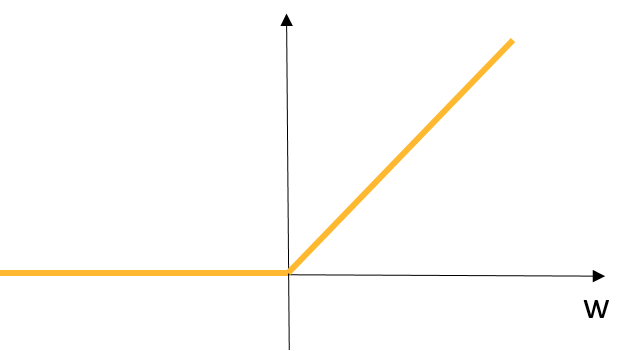
\includegraphics[width=0.32\linewidth]{Dissertation/images/ch1/bayesian_classifier_approximation/relu.png}}
        \hfill
        \subcaptionbox{LeakyReLU(w) = \(max(0.01w, w)\)}{%
            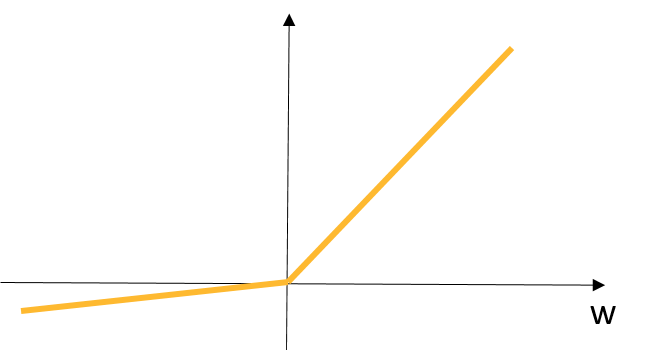
\includegraphics[width=0.32\linewidth]{Dissertation/images/ch1/bayesian_classifier_approximation/leaky_relu.png}}
        \hfill
        \subcaptionbox{Abs(w) = \(|w|\)}{%
            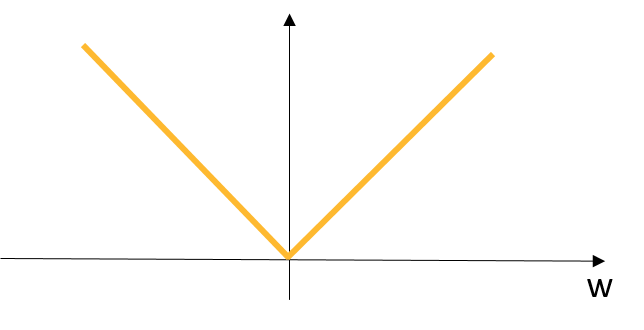
\includegraphics[width=0.32\linewidth]{Dissertation/images/ch1/bayesian_classifier_approximation/abs.png}}
        \hfill
    }
    \caption{Кусочно-линейные функции активации}
    \label{fig:activations}
\end{figure}

Пусть выборка \((X, Y)\) имеет на \(\mathbb{S}\) равномерно непрерывную плотность \(f(X)\):

\[
    f(X) = p_{-1} f_{-1}(X) + p_{+1} f_{+1}(X),
\]

\noindent где \(f_{-1}\) и \(f_{+1}\) -- плотности классов \(-1\) и \(+1\) соответственно.

Для формирования выборки из смеси реальных данных и ``фона`` с плотностью \(\alpha f(X) + (1 - \alpha) p(X)\) добавим к этой выборке искуственно сгенерированные данные \(\{(X_{n+1}, Y_{n+1}), \dots, (X_{2n}, Y_{2n})\}\), где векторы \(\{X_{n+1}, \dots, X_{2n}\}\) -- наблюдения независимо равномерно распределённых на \([0, 1]^d\) случайных векторов c плотностью \(p(X)\), а \(Y_{n+i} = 0, i=1..n\).

Пусть \(C(L, k)\) -- множество всех многослойных персептронов \(c(X)\) с одним нейроном с линейной функцией активации в выходном слое, кусочно-линейной функцией активации \(|\cdot|\) (модульная) в скрытых слоях и числом \(L\) и размером \(k\) скрытых слоёв.

\nomenclature{\(C(L, k)\)}{множество всех многослойных персептронов \(c(X)\) с одним нейроном с линейной функцией активации в выходном слое, кусочно-линейной функцией активации \(|\cdot|\) в скрытых слоях и числом \(L\) и размером \(k\) скрытых слоёв}

Применяя некоторый алгоритм оптимизации (градиентный спуск~\cite{amari1993backpropagation}, генетический алгоритм~\cite{seiffert2001multiple} и т.д.), построим выборочную оценку решения задачи~\cref{eq:regression_approx}:

\begin{equation}
    \label{eq:perceptron_optimization}
    \sum\limits_{i=1}^{2n} (c_n(X_i) - Y_i)^2 \rightarrow \min\limits_{c_n(X)\in C(L, k)},
\end{equation}

\noindent где параметры \(L\) и \(k\) выбраны оптимально с учётом ограничений, связанных с переобучением.

Пусть функция \(c_n^*(X)\) -- решение оптимизационной задачи~\cref{eq:perceptron_optimization}, которая в дальнейшем будет называться \textbf{функцией нейросетевой регрессии}. Соответствующий этому решению персептрон строит иерархическое (по слоям) разбиение компакта \([0, 1]^d\) на \(O(k^{dL})\) непересекающихся ячеек~\cite{devroye2013probabilistic} (при \(k > d\)).

\nomenclature{\(c_n^*(X)\)}{функция нейросетевой регрессии}

\begin{figure}[ht]
    \centerfloat{
        \hfill
        \subcaptionbox{Ячейки первого слоя: 18}{%
            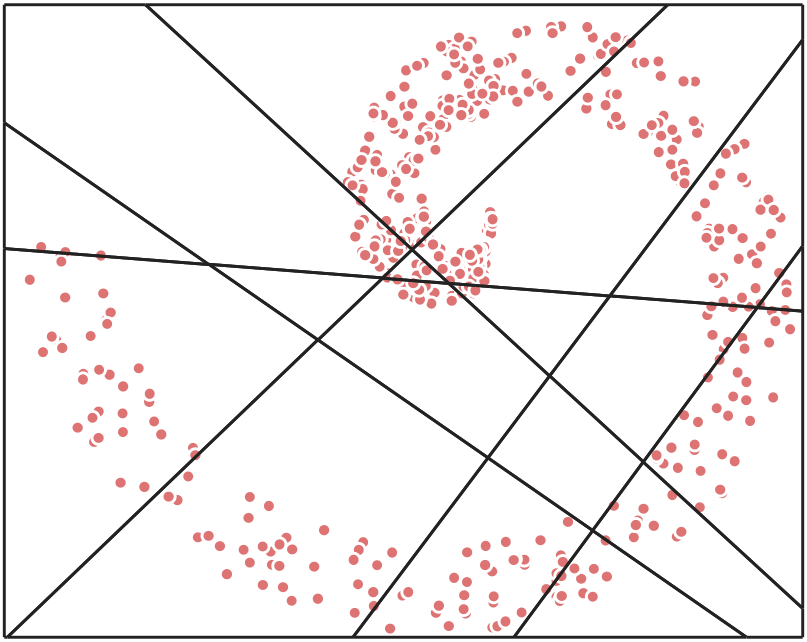
\includegraphics[width=0.3\linewidth]{Dissertation/images/ch1/bayesian_classifier_approximation/partition_l1.png}}
        \hfill
        \subcaptionbox{Ячейки второго слоя: 121}{%
            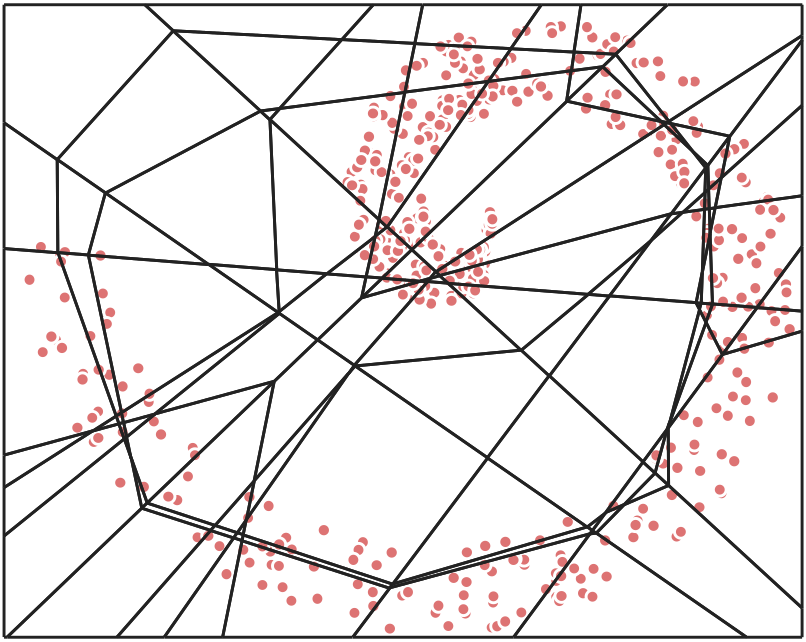
\includegraphics[width=0.3\linewidth]{Dissertation/images/ch1/bayesian_classifier_approximation/partition_l2.png}}
        \hfill
        \subcaptionbox{Ячейки выходного слоя: 148}{%
            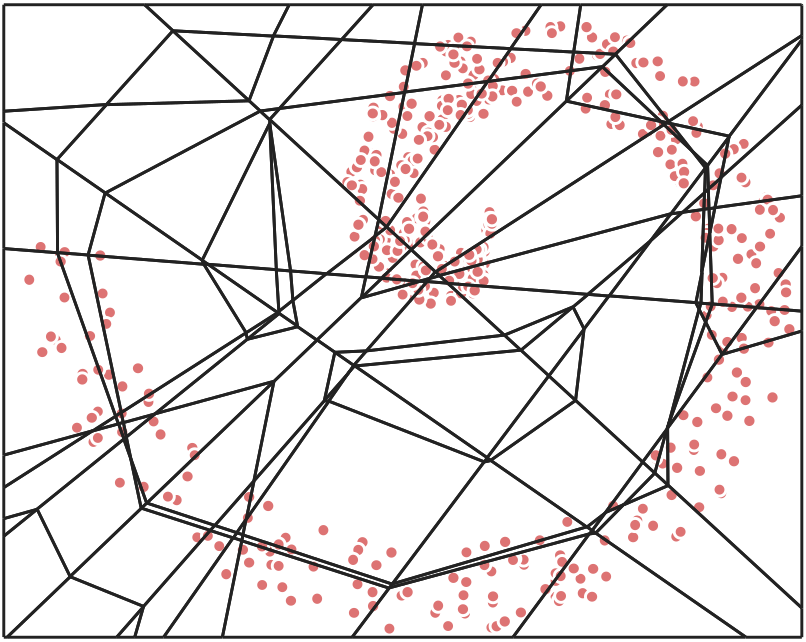
\includegraphics[width=0.3\linewidth]{Dissertation/images/ch1/bayesian_classifier_approximation/partition_l3.png}}
        \hfill
    }
    \caption{Пример разбиения некоторым персептроном с \(L=2\), \(k=6\)}
    \label{fig:perceptron_partition}
\end{figure}

Пример такого разбиения показан на рисунке~\cref{fig:perceptron_partition}, где персептрон имеет \(L=2\) скрытых слоя по \(k=6\) нейронов.

%%%%%%%%%%%%%%%%%%%%%%%%%%%%%%%%%%%%%%%%%%%%%%%%%%%%%%%%%%%%%%%%%%%%%%%%%%%%%%%%%%%%%%%%%%%%%%%%%%%%%%%%%%%%%%%
\subsection{Адаптивная гистограммная аппроксимация}\label{subsec:ch1/histogram_approximation}

Пусть в результате построения \(c_n^*(X)\) получено разбиение компакта \([0, 1]^d\) на \(N\) непересекающихся ячеек \(\{K_1, K_2, \dots, K_N\}\). Рассмотрим кусочно-постоянную (в общем случае разрывную) \textbf{функцию гистограммной регрессии} \(h_n(X)\), принимающую постоянные значения в ячейках разбиения \([0, 1]^d\) и решим для неё оптимизационную задачу:

\nomenclature{\(h_n^*(X)\)}{функция гистограммной регрессии}

\begin{equation}
    \label{eq:histogram_optimization}
    \sum\limits_{i=1}^{2n} (h_n(X_i) - Y_i)^2 \rightarrow \min\limits_{h_n(X)},
\end{equation}

Пусть \(X \in K_r\). Тогда задачу~\cref{eq:histogram_optimization} для этой ячейки можно представить в следующем виде:

\nomenclature{\(K_r\)}{некоторая ячейка из разбиения компакта \([0,1]^d\)}

\begin{equation}
    \label{eq:histogram_cell_optimization}
    n_{-1}(X)\cdot(h_n(X) + 1)^2 + n_0(X)\cdot(h_n(X) - 0)^2 + n_{+1}(X)\cdot(h_n(X) - 1)^2 \rightarrow \min\limits_{h_n(X)},
\end{equation}

\noindent где \(n_j = \sum\limits_{i=1}^{2n} I_{X_i \in K_r, Y_i = j}\).

После дифференцирования функции~\cref{eq:histogram_cell_optimization} по \(h_n(X)\) получаем решение задачи~\cref{eq:histogram_optimization}:

\begin{equation}
    \label{eq:histogram_cell_solution}
    h_n^*(X) = \frac{n_{+1}(X) - n_{-1}(X)}{n_{-1}(X) + n_0(X) + n_{+1}(X)}.
\end{equation}

Пример вычисления функции гистограммной регрессии показан на рисунке~\cref{fig:histogram_evaluation}.

\fixme{ЗАМЕНИТЬ РИСУНОК}
\begin{figure}[ht]
    \centerfloat{
        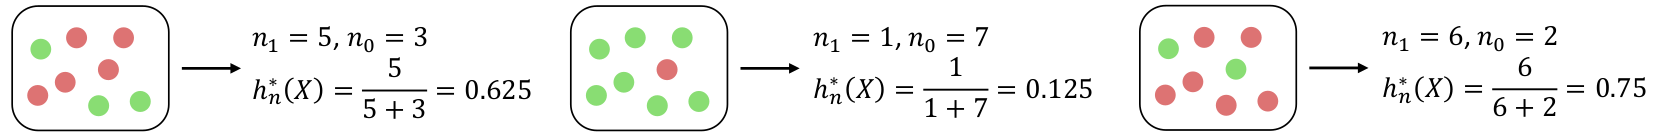
\includegraphics[width=\linewidth]{Dissertation/images/ch1/bayesian_classifier_approximation/histogram_evaluation.png}
    }
    \caption{Пример вычисления \(h_n^*(X)\) в некоторой ячейке \(K_r\)}
    \label{fig:histogram_evaluation}
\end{figure}

Основными достоинствами использования такой аппроксимации являются независимость от масштаба и отсутствие необходимости введения метрик, как того требуют методы на основе расстояний вроде \(k\) ближайших соседей.